\documentclass{article}

\usepackage[utf8]{inputenc}
\usepackage[dvipsnames]{xcolor}
\usepackage{lmodern}
\usepackage{graphicx}
\usepackage{longtable}
\usepackage{tabularx}

\graphicspath{ {../images/} }
\usepackage{imakeidx}
\makeindex[columns=3, title=Alphabetical Index, intoc]

\usepackage{tabularx}
\usepackage{amsmath}
\usepackage{paralist}
\usepackage{enumitem}
\usepackage{hyperref} %\usepackage[hidelinks]{hyperref} %per togliere bordi rossi
\usepackage{makecell}
\usepackage{caption}
\usepackage[maxfloats=256]{morefloats}
\maxdeadcycles=1000

\usepackage[official]{eurosym}

\DeclareUnicodeCharacter{20AC}{\euro{}}

\author{Agosta, Belli, Emili, Giacchini, Luciani}

\begin{document}

\begin{center}
    \sffamily{\fontsize{50}{48} \selectfont \textcolor{red}{Nexi}\textcolor{green}{Fy}}
\end{center}

\begin{center}
    \itshape{\fontsize{20}{48} \selectfont streaming to your pocket}
\end{center}

\bigskip\bigskip\bigskip

\begin{flushleft}
    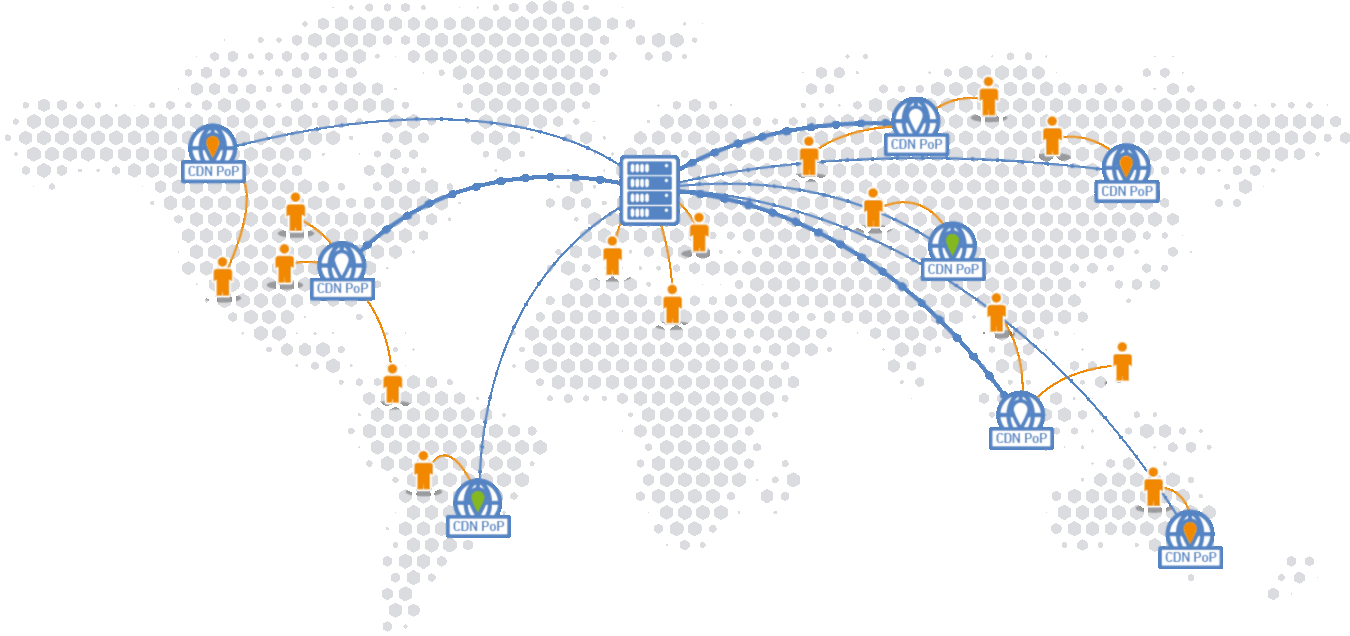
\includegraphics[scale=1]{../images/worldCDN.png}
\end{flushleft}

\bigskip\bigskip\bigskip

\begin{center}
    \itshape{\fontsize{30}{48} \selectfont Analisi del sistema}
\end{center}

\newpage
\printindex

\newpage
\section{\itshape{Analisi del sistema}}

\subsection{Analisi Nomi-Verbi}
Viene qui rappresentato l’elenco delle funzionalità che il sistema deve avere, sulla base dal Documento di Visione.
Inoltre, sono presenti le definizioni necessarie.
La legenda spiega come interpretare le informazioni.

\subsubsection{Legenda}

\begin{itemize}
    \item Nomi propri: istanze;
    \item Nomi comuni o predicati nominali: \textcolor{red}{classi} o \textcolor{orange}{attributi};
    %\item \textcolor{teal}{Verbi transitivi}: metodi;
    \item \textcolor{teal}{Verbi}: metodi;
    \item \textcolor{cyan}{Verbi modali}: precondizioni, postcondizioni, o condizioni di invarianza;
    %\item \textcolor{blue}{Verbi intransitivi}: eccezioni o eventi dipendenti dal tempo;
    \item \textcolor{violet}{Aggettivi}: valore di attributo o classe;
    \item  \underline{Riferimenti} alle definizioni.
\end{itemize}

\subsubsection{Definizioni}
\begin{enumerate}
    \item \textcolor{red}{Utente del sistema}: fornito di informazioni riguardanti \textcolor{orange}{nome}, \textcolor{orange}{cognome},
    \textcolor{orange}{data di nascita}, \textcolor{orange}{email}, \textcolor{orange}{password}, \textcolor{orange}{metodi di pagamento}
    Ha la possibilità di sottoscrivere \textcolor{red}{abbonamenti}. Un \textcolor{red}{partner} è un \textcolor{red}{utente} con un \textcolor{red}{abbonamento} che gli consente di pubblicare sulla piattaforma;
    \item \textcolor{red}{Piano di abbonamento}: selezionabile dagli utenti, ha proprietà quali \textcolor{orange}{nome},
    \textcolor{orange}{prezzo}, \textcolor{orange}{durata}, \textcolor{orange}{disponibilità di sottoscrizione}.
    Esso raggruppa una lista di \textcolor{red}{servizi} \textcolor{teal}{offerti};
    \item \textcolor{red}{Servizio}: caratterizzato da \textcolor{orange}{ID} e \textcolor{orange}{descrizione};
    \item \textcolor{red}{Prodotto multimediale}: oltre agli elementi identificativi, è caratterizzato da\textcolor{orange}{genere},
    \textcolor{orange}{visibilità}, \textcolor{red}{utente} \textcolor{orange}{proprietario}. Esso può essere di tipo
    \textcolor{red}{video} o \textcolor{red}{audio}: nel primo caso è fornito di \textcolor{orange}{traccia audio} e
    \textcolor{orange}{traccia video}, nel secondo solo \textcolor{orange}{traccia audio}, ma con accompagnamento di
    \textcolor{orange}{lyrics} o \textcolor{orange}{video musicale};
    \item \textcolor{red}{Playlist}: contenente una lista di \textcolor{red}{prodotti multimediali}.\\
    Casi particolari di essa sono:
    \begin{enumerate}
        \item \textcolor{red}{Serie TV}: formata solamente da \textcolor{violet}{prodotti video}, tutti pubblicati dallo stesso \textcolor{red}{utente};
        \item \textcolor{red}{Album}: formato solamente da \textcolor{violet}{prodotti audio}, tutti pubblicati dallo stesso \textcolor{red}{utente};
    \end{enumerate}
    \item \textcolor{red}{Visualizzazione}: proveniente da un \textcolor{red}{utente} verso un \textcolor{red}{prodotto multimediale},
    considera anche l'\textcolor{orange}{istante} in cui avviene;
    \item \textcolor{red}{Segnalazione}: relativa ad un \textcolor{red}{prodotto multimediale}, caratterizzata dall' \textcolor{red}{utente} che 
    la effettua e una \textcolor{orange}{motivazione};
    \item \textcolor{red}{Coda di riproduzione}: relativa ad un singolo \textcolor{red}{utente}, composta da una lista di  
    \textcolor{red}{prodotti multimediali};
    \item \textcolor{red}{Amministratore del sistema}: \textcolor{teal}{si occupa} della gestione del sistema;
    \item \textcolor{red}{Valutazione}: relative a contenuti e \textcolor{teal}{create} da \textcolor{red}{utenti};
\end{enumerate}

\subsubsection{Funzionalità}
\begin{enumerate}
    \item L' \textcolor{red}{amministratore} \textcolor{teal}{effettua} diverse operazioni sugli \textcolor{red}{abbonamenti}.
    Egli \textcolor{teal}{crea} \textcolor{red}{abbonamenti} e \textcolor{cyan}{può} \textcolor{teal}{attivare} e
    \textcolor{teal}{disattivare} alcuni già \textcolor{violet}{creati}, \textcolor{teal}{modificando} la loro \textcolor{orange}{disponibilità}.
    Inoltre, egli \textcolor{teal}{aggiunge} e \textcolor{teal}{rimuove} \textcolor{red}{servizi} da \textcolor{red}{abbonamenti}.
    L' \textcolor{red}{amministratore} \textcolor{cyan}{può} anche \textcolor{teal}{recuperare} \textcolor{orange}{informazioni} riguardanti
    \textcolor{red}{servizi} (\textcolor{violet}{generici} o in un particolare \textcolor{red}{abbonamento}) e \textcolor{red}{piani di abbonamento};
    \item Il sistema \textcolor{teal}{effettua} pagamenti verso i \textcolor{red}{partner}.
    \item L' \textcolor{red}{amministratore} \textcolor{cyan}{può} \textcolor{teal}{sospendere} l'account di un \textcolor{red}{utente};
    \item L' \textcolor{red}{utente} \textcolor{teal}{effettua} operazioni sul proprio account. Egli \textcolor{teal}{si registra},
    \textcolor{teal}{fornendo} i propri dati, \textcolor{teal}{modifica} il proprio profilo ed \textcolor{teal}{effettua}
    login e logout per \textcolor{teal}{autenticarsi} sulla piattaforma.
    \item L' \textcolor{red}{utente} \textcolor{teal}{richiede} ricerche al sistema. Queste sono relative
    ad un particolare contenuto (\textcolor{red}{prodotto} o \textcolor{red}{playlist}) oppure indirizzate a contenuti
    \textcolor{violet}{popolari}. Inoltre, il sistema \textcolor{teal}{suggerisci} contenuti agli
    \textcolor{red}{utenti}, sulla base delle loro \textcolor{orange}{preferenze};
    \item L' \textcolor{red}{utente} \textcolor{teal}{sottoscrive} nuovi \textcolor{red}{abbonamenti} e ne \textcolor{teal}{disdice} di già
    \textcolor{orange}{sottoscritti}. Egli \textcolor{cyan}{può} \textcolor{teal}{cambiare} un \textcolor{red}{abbonamento} con un altro,
    pagando eventualmente un sovrapprezzo. Il sistema \textcolor{teal}{gestisce} il rinnovo automatico;
    \item Il \textcolor{red}{partner} \textcolor{teal}{pubblica} nuovi \textcolor{red}{prodotti} sulla piattaforma. Egli \textcolor{teal}{compila}
    le \textcolor{orange}{informazioni di base}. Inoltre, nel caso di un 
    \textcolor{red}{prodotto video}, egli \textcolor{teal}{carica} il file video, il file audio e \textcolor{violet}{opzionalmente} sottotitoli.
    Invece, per un \textcolor{red}{prodotto audio}, egli \textcolor{teal}{carica} il file audio e \textcolor{violet}{opzionalmente} video musicale o lyrics.
    Egli, \textcolor{cyan}{può} anche \textcolor{teal}{cambiare} lo stato della pubblicazione, tra \textcolor{violet}{pubblico} e \textcolor{violet}{privato};
    \item L' \textcolor{red}{utente} \textcolor{teal}{riproduce} \textcolor{red}{prodotti} (sia video che audio) con il player. Egli \textcolor{cyan}{può} \textcolor{teal}{mettere}
    il player \textcolor{violet}{in pausa} e \textcolor{violet}{in riproduzione} e \textcolor{teal}{spostare} il punto di riproduzione. 
    Egli \textcolor{cyan}{può} anche \textcolor{teal}{riprodurre} audio in background;
    \item L' \textcolor{red}{utente} \textcolor{teal}{effettua} operazioni sulle \textcolor{red}{playlist}. Egli crea nuove \textcolor{red}{playlist}, \textcolor{violet}{vuote};
    \textcolor{teal}{aggiunge} e \textcolor{teal}{rimuove} \textcolor{red}{prodotti} ad/da esse;  \textcolor{teal}{cambia} la loro \textcolor{orange}{visibilità} (\textcolor{violet}{pubblica} o \textcolor{violet}{privata});
    \textcolor{teal}{riproduce} playlist, che \textcolor{cyan}{devono}  \textcolor{teal}{contenere} almeno un  \textcolor{red}{prodotto};
    \item Il \textcolor{red}{partner} \textcolor{teal}{crea} una \textcolor{red}{serie TV};
    \item Il \textcolor{red}{partner} \textcolor{teal}{crea} un \textcolor{red}{album};
    \item L' \textcolor{red}{utente} \textcolor{cyan}{può} \textcolor{teal}{valutare} contenuti. Egli \textcolor{cyan}{può} \textcolor{teal}{votare} il contenuto
    e/o  \textcolor{teal}{commentarlo}. Il commento \textcolor{cyan}{può} \textcolor{teal}{essere eliminato} dallo stesso \textcolor{red}{utente};
    \item L' \textcolor{red}{utente} \textcolor{cyan}{può} \textcolor{teal}{segnalare} \textcolor{red}{prodotti} e l' \textcolor{red}{amministratore} \textcolor{teal}{controllare} le 
    \textcolor{red}{segnalazioni} di un certo \textcolor{red}{utente};
    \item L' \textcolor{red}{utente} \textcolor{teal}{ottiene} la cronologia dei contenuti visualizzati;
    \item L' \textcolor{red}{utente} \textcolor{teal}{effettua} il download di un certo \textcolor{red}{prodotto};
    \item L' \textcolor{red}{utente} \textcolor{teal}{riproduce} spot pubblicitari.
    \item Il sistema \textcolor{teal}{calcola} il voto di un certo contenuto, sulla base dei voti ricevuti.
    \item L' \textcolor{red}{utente} \textcolor{teal}{effettua} operazioni sulla \textcolor{red}{coda di riproduzione}. Egli \textcolor{teal}{aggiunge}
    e \textcolor{teal}{rimuove} \textcolor{red}{prodotti} da essa. Inoltre, egli \textcolor{cyan}{può} \textcolor{teal}{visualizzare} i 
    \textcolor{red}{prodotti} presenti nella \textcolor{red}{coda}.
\end{enumerate}


%============================ SCHEDE CRC =====================================

\subsection{Schede CRC - Class-Responsability-Collaboration}

Che cosa sono\\

\begin{center}
    \begin{tabular}{ |p{3cm}|p{3cm}|p{3cm}|p{3cm}| }
        \hline
        Nome & \multicolumn{3}{|p{9cm}|}{Amministratore} \\\hline
        SuperClassi & \multicolumn{3}{|p{9cm}|}{-} \\\hline
        SottoClassi & \multicolumn{3}{|p{9cm}|}{ManagerAbbonamenti, ManagerSegnalazioni} \\\hline
        Attributi & \multicolumn{3}{|p{9cm}|}{nome,cognome,codice fiscale, recapito telefonico} \\\hline
        \multicolumn{4}{|p{12cm}|}{Responsabilit\'a} \\\hline
        \multicolumn{2}{|p{6cm}|}{Nome} & \multicolumn{2}{|p{6cm}|}{Collaboratore} \\\hline
        \multicolumn{4}{|p{12cm}|}{-} \\\hline
    \end{tabular}
\end{center}

\begin{center}
    \begin{tabular}{ |p{3cm}|p{3cm}|p{3cm}|p{3cm}| }
        \hline
        Nome & \multicolumn{3}{|p{9cm}|}{ManagerAbbonamenti} \\\hline
        SuperClassi & \multicolumn{3}{|p{9cm}|}{Amministratore} \\\hline
        SottoClassi & \multicolumn{3}{|p{9cm}|}{-} \\\hline
        Attributi & \multicolumn{3}{|p{9cm}|}{-} \\\hline
        \multicolumn{4}{|p{12cm}|}{Responsabilit\'a} \\\hline
        \multicolumn{2}{|p{6cm}|}{Nome} & \multicolumn{2}{|p{6cm}|}{Collaboratore} \\\hline
        \multicolumn{2}{|p{6cm}|}{gestire gli abbonamenti} & \multicolumn{2}{|p{6cm}|}{handlerAbbonamenti} \\\hline
        \multicolumn{2}{|p{6cm}|}{gestire servizi} & \multicolumn{2}{|p{6cm}|}{handlerServizi} \\\hline
    \end{tabular}
\end{center}

\begin{center}
    \begin{tabular}{ |p{3cm}|p{3cm}|p{3cm}|p{3cm}| }
        \hline
        Nome & \multicolumn{3}{|p{9cm}|}{ManagerSegnalazioni} \\\hline
        SuperClassi & \multicolumn{3}{|p{9cm}|}{Amministratore} \\\hline
        SottoClassi & \multicolumn{3}{|p{9cm}|}{-} \\\hline
        Attributi & \multicolumn{3}{|p{9cm}|}{-} \\\hline
        \multicolumn{4}{|p{12cm}|}{Responsabilit\'a} \\\hline
        \multicolumn{2}{|p{6cm}|}{Nome} & \multicolumn{2}{|p{6cm}|}{Collaboratore} \\\hline
        \multicolumn{2}{|p{6cm}|}{gestire le segnalazioni} & \multicolumn{2}{|p{6cm}|}{handlerSegnalazioni} \\\hline
        \multicolumn{2}{|p{6cm}|}{gestire sospensioni account utente} & \multicolumn{2}{|p{6cm}|}{handlerUserBan} \\\hline
        \multicolumn{2}{|p{6cm}|}{gestire sospensioni risorse segnalate} & \multicolumn{2}{|p{6cm}|}{handlerProductBan} \\\hline
    \end{tabular}
\end{center}

\begin{center}
    \begin{tabular}{ |p{3cm}|p{3cm}|p{3cm}|p{3cm}| }
        \hline
        Nome & \multicolumn{3}{|p{9cm}|}{Utente} \\\hline
        SuperClassi & \multicolumn{3}{|p{9cm}|}{-} \\\hline
        SottoClassi & \multicolumn{3}{|p{9cm}|}{UtenteNonAutenticato, UtenteAutenticato} \\\hline
        Attributi & \multicolumn{3}{|p{9cm}|}{-} \\\hline
        \multicolumn{4}{|p{12cm}|}{Responsabilit\'a} \\\hline
        \multicolumn{2}{|p{6cm}|}{Nome} & \multicolumn{2}{|p{6cm}|}{Collaboratore} \\\hline
        \multicolumn{2}{|p{6cm}|}{richiede una ricerca} & \multicolumn{2}{|p{6cm}|}{handlerRicerche} \\\hline
        \multicolumn{2}{|p{6cm}|}{ottenere cronologia prodotti visualizzati/ascoltati} & \multicolumn{2}{|p{6cm}|}{handlerRicerche} \\\hline
    \end{tabular}
\end{center}

\begin{center}
    \begin{longtable}{ |p{3cm}|p{3cm}|p{3cm}|p{3cm}| }
        \hline
        Nome & \multicolumn{3}{|p{9cm}|}{UtenteAutenticato} \\\hline
        SuperClassi & \multicolumn{3}{|p{9cm}|}{Utente} \\\hline
        SottoClassi & \multicolumn{3}{|p{9cm}|}{Partner} \\\hline
        Attributi & \multicolumn{3}{|p{9cm}|}{nome, cognome, data di nascita, email, password, email di recupero, data di registrazione, metodo di pagamento, stato, abbonamenti sottoscritti, attivo } \\\hline
        \multicolumn{4}{|p{12cm}|}{Responsabilit\'a} \\\hline
        \multicolumn{2}{|p{6cm}|}{Nome} & \multicolumn{2}{|p{6cm}|}{Collaboratore} \\\hline
        \multicolumn{2}{|p{6cm}|}{effettua login} & \multicolumn{2}{|p{6cm}|}{handlerLogin} \\\hline
        \multicolumn{2}{|p{6cm}|}{effettua logout} & \multicolumn{2}{|p{6cm}|}{handlerLogout} \\\hline
        \multicolumn{2}{|p{6cm}|}{modifica i propri dati} & \multicolumn{2}{|p{6cm}|}{handlerProfilo} \\\hline
        \multicolumn{2}{|p{6cm}|}{sottoscrive abbonamenti} & \multicolumn{2}{|p{6cm}|}{handlerAbbonamenti} \\\hline
        \multicolumn{2}{|p{6cm}|}{disdice abbonamenti} & \multicolumn{2}{|p{6cm}|}{handlerAbbonamenti} \\\hline
        \multicolumn{2}{|p{6cm}|}{cambia abbonamenti} & \multicolumn{2}{|p{6cm}|}{handlerAbbonamenti} \\\hline
        \multicolumn{2}{|p{6cm}|}{creare playlist} & \multicolumn{2}{|p{6cm}|}{handlerPlaylist} \\\hline
        \multicolumn{2}{|p{6cm}|}{modifica le proprie playlist} & \multicolumn{2}{|p{6cm}|}{handlerPlaylist} \\\hline
        \multicolumn{2}{|p{6cm}|}{valutare prodotto} & \multicolumn{2}{|p{6cm}|}{handlerValutazioni} \\\hline
        \multicolumn{2}{|p{6cm}|}{modificare valutazione a un prodotto} & \multicolumn{2}{|p{6cm}|}{handlerValutazioni} \\%\hline
        \multicolumn{2}{|p{6cm}|}{segnalare un prodotto} & \multicolumn{2}{|p{6cm}|}{handlerSegnalazioni} \\\hline
        \multicolumn{2}{|p{6cm}|}{scaricare prodotto} & \multicolumn{2}{|p{6cm}|}{handlerDownload} \\\hline
        \multicolumn{2}{|p{6cm}|}{riprodurre prodotti} & \multicolumn{2}{|p{6cm}|}{handlerRiproduzione} \\\hline
        \multicolumn{2}{|p{6cm}|}{interagire con player} & \multicolumn{2}{|p{6cm}|}{handlerPlayer} \\\hline
        \multicolumn{2}{|p{6cm}|}{riprodurre prodotti in background} & \multicolumn{2}{|p{6cm}|}{handlerRiproduzione} \\\hline
        \multicolumn{2}{|p{6cm}|}{riprodurre playlist} & \multicolumn{2}{|p{6cm}|}{handlerRiproduzione} \\\hline
        \multicolumn{2}{|p{6cm}|}{riproduce una pubblicità} & \multicolumn{2}{|p{6cm}|}{handlerRiproduzione} \\\hline
        \multicolumn{2}{|p{6cm}|}{gestire coda riproduzione} & \multicolumn{2}{|p{6cm}|}{handlerCodaRiproduzione} \\\hline
    \end{longtable}
\end{center}

\begin{center}
    \begin{tabular}{ |p{3cm}|p{3cm}|p{3cm}|p{3cm}| }
        \hline
        Nome & \multicolumn{3}{|p{9cm}|}{UtenteNonAutenticato} \\\hline
        SuperClassi & \multicolumn{3}{|p{9cm}|}{Utente} \\\hline
        SottoClassi & \multicolumn{3}{|p{9cm}|}{-} \\\hline
        Attributi & \multicolumn{3}{|p{9cm}|}{- } \\\hline
        \multicolumn{4}{|p{12cm}|}{Responsabilit\'a} \\\hline
        \multicolumn{2}{|p{6cm}|}{Nome} & \multicolumn{2}{|p{6cm}|}{Collaboratore} \\\hline
        \multicolumn{2}{|p{6cm}|}{richiede la registrazione} & \multicolumn{2}{|p{6cm}|}{handlerRegistrazione} \\\hline
    \end{tabular}
\end{center}

\begin{center}
    \begin{tabular}{ |p{3cm}|p{3cm}|p{3cm}|p{3cm}| }
        \hline
        Nome & \multicolumn{3}{|p{9cm}|}{Partner} \\\hline
        SuperClassi & \multicolumn{3}{|p{9cm}|}{UtenteAutenticato} \\\hline
        SottoClassi & \multicolumn{3}{|p{9cm}|}{-} \\\hline
        Attributi & \multicolumn{3}{|p{9cm}|}{metodo di ricezione pagamenti } \\\hline
        \multicolumn{4}{|p{12cm}|}{Responsabilit\'a} \\\hline
        \multicolumn{2}{|p{6cm}|}{Nome} & \multicolumn{2}{|p{6cm}|}{Collaboratore} \\\hline
        \multicolumn{2}{|p{6cm}|}{pubblica prodotti} & \multicolumn{2}{|p{6cm}|}{handlerProdotti} \\\hline
        \multicolumn{2}{|p{6cm}|}{modifica prodotti} & \multicolumn{2}{|p{6cm}|}{handlerProdotti} \\\hline
        \multicolumn{2}{|p{6cm}|}{creare una serie TV} & \multicolumn{2}{|p{6cm}|}{handlerPlaylist} \\\hline
        \multicolumn{2}{|p{6cm}|}{creare un Album} & \multicolumn{2}{|p{6cm}|}{handlerPlaylist} \\\hline
    \end{tabular}
\end{center}

\begin{center}
    \begin{tabular}{ |p{3cm}|p{3cm}|p{3cm}|p{3cm}| }
        \hline
        Nome & \multicolumn{3}{|p{9cm}|}{Contenuto} \\\hline
        SuperClassi & \multicolumn{3}{|p{9cm}|}{-} \\\hline
        SottoClassi & \multicolumn{3}{|p{9cm}|}{Prodotto, Playlist} \\\hline
        Attributi & \multicolumn{3}{|p{9cm}|}{titolo, descrizione, visibilità, proprietario} \\\hline
        \multicolumn{4}{|p{12cm}|}{Responsabilit\'a} \\\hline
        \multicolumn{2}{|p{6cm}|}{Nome} & \multicolumn{2}{|p{6cm}|}{Collaboratore} \\\hline
        \multicolumn{2}{|p{6cm}|}{-} & \multicolumn{2}{|p{6cm}|}{-} \\\hline
    \end{tabular}
\end{center}

\begin{center}
    \begin{tabular}{ |p{3cm}|p{3cm}|p{3cm}|p{3cm}| }
        \hline
        Nome & \multicolumn{3}{|p{9cm}|}{Prodotto} \\\hline
        SuperClassi & \multicolumn{3}{|p{9cm}|}{Contenuto} \\\hline
        SottoClassi & \multicolumn{3}{|p{9cm}|}{ProdottoVideo, ProdottoAudio} \\\hline
        Attributi & \multicolumn{3}{|p{9cm}|}{età minima, genere} \\\hline
        \multicolumn{4}{|p{12cm}|}{Responsabilit\'a} \\\hline
        \multicolumn{2}{|p{6cm}|}{Nome} & \multicolumn{2}{|p{6cm}|}{Collaboratore} \\\hline
        \multicolumn{2}{|p{6cm}|}{-} & \multicolumn{2}{|p{6cm}|}{-} \\\hline
    \end{tabular}
\end{center}

\begin{center}
    \begin{tabular}{ |p{3cm}|p{3cm}|p{3cm}|p{3cm}| }
        \hline
        Nome & \multicolumn{3}{|p{9cm}|}{ProdottoVideo} \\\hline
        SuperClassi & \multicolumn{3}{|p{9cm}|}{Prodotto} \\\hline
        SottoClassi & \multicolumn{3}{|p{9cm}|}{-} \\\hline
        Attributi & \multicolumn{3}{|p{9cm}|}{file video, file audio, sottotitoli} \\\hline
        \multicolumn{4}{|p{12cm}|}{Responsabilit\'a} \\\hline
        \multicolumn{2}{|p{6cm}|}{Nome} & \multicolumn{2}{|p{6cm}|}{Collaboratore} \\\hline
        \multicolumn{2}{|p{6cm}|}{-} & \multicolumn{2}{|p{6cm}|}{-} \\\hline
    \end{tabular}
\end{center}

\begin{center}
    \begin{tabular}{ |p{3cm}|p{3cm}|p{3cm}|p{3cm}| }
        \hline
        Nome & \multicolumn{3}{|p{9cm}|}{ProdottoAudio} \\\hline
        SuperClassi & \multicolumn{3}{|p{9cm}|}{Prodotto} \\\hline
        SottoClassi & \multicolumn{3}{|p{9cm}|}{-} \\\hline
        Attributi & \multicolumn{3}{|p{9cm}|}{file audio, file lyrics, file video musicale} \\\hline
        \multicolumn{4}{|p{12cm}|}{Responsabilit\'a} \\\hline
        \multicolumn{2}{|p{6cm}|}{Nome} & \multicolumn{2}{|p{6cm}|}{Collaboratore} \\\hline
        \multicolumn{2}{|p{6cm}|}{-} & \multicolumn{2}{|p{6cm}|}{-} \\\hline
    \end{tabular}
\end{center}

\begin{center}
    \begin{tabular}{ |p{3cm}|p{3cm}|p{3cm}|p{3cm}| }
        \hline
        Nome & \multicolumn{3}{|p{9cm}|}{Playlist} \\\hline
        SuperClassi & \multicolumn{3}{|p{9cm}|}{Contenuto} \\\hline
        SottoClassi & \multicolumn{3}{|p{9cm}|}{SerieTv, Album} \\\hline
        Attributi & \multicolumn{3}{|p{9cm}|}{prodotti} \\\hline
        \multicolumn{4}{|p{12cm}|}{Responsabilit\'a} \\\hline
        \multicolumn{2}{|p{6cm}|}{Nome} & \multicolumn{2}{|p{6cm}|}{Collaboratore} \\\hline
        \multicolumn{2}{|p{6cm}|}{-} & \multicolumn{2}{|p{6cm}|}{-} \\\hline
    \end{tabular}
\end{center}

\begin{center}
    \begin{tabular}{ |p{3cm}|p{3cm}|p{3cm}|p{3cm}| }
        \hline
        Nome & \multicolumn{3}{|p{9cm}|}{SerieTv} \\\hline
        SuperClassi & \multicolumn{3}{|p{9cm}|}{Playlist} \\\hline
        SottoClassi & \multicolumn{3}{|p{9cm}|}{-} \\\hline
        Attributi & \multicolumn{3}{|p{9cm}|}{genere} \\\hline
        \multicolumn{4}{|p{12cm}|}{Responsabilit\'a} \\\hline
        \multicolumn{2}{|p{6cm}|}{Nome} & \multicolumn{2}{|p{6cm}|}{Collaboratore} \\\hline
        \multicolumn{2}{|p{6cm}|}{-} & \multicolumn{2}{|p{6cm}|}{-} \\\hline
    \end{tabular}
\end{center}

\begin{center}
    \begin{tabular}{ |p{3cm}|p{3cm}|p{3cm}|p{3cm}| }
        \hline
        Nome & \multicolumn{3}{|p{9cm}|}{Album} \\\hline
        SuperClassi & \multicolumn{3}{|p{9cm}|}{Playlist} \\\hline
        SottoClassi & \multicolumn{3}{|p{9cm}|}{-} \\\hline
        Attributi & \multicolumn{3}{|p{9cm}|}{genere} \\\hline
        \multicolumn{4}{|p{12cm}|}{Responsabilit\'a} \\\hline
        \multicolumn{2}{|p{6cm}|}{Nome} & \multicolumn{2}{|p{6cm}|}{Collaboratore} \\\hline
        \multicolumn{2}{|p{6cm}|}{-} & \multicolumn{2}{|p{6cm}|}{-} \\\hline
    \end{tabular}
\end{center}

\begin{center}
    \begin{tabular}{ |p{3cm}|p{3cm}|p{3cm}|p{3cm}| }
        \hline
        Nome & \multicolumn{3}{|p{9cm}|}{Visualizzazione} \\\hline
        SuperClassi & \multicolumn{3}{|p{9cm}|}{-} \\\hline
        SottoClassi & \multicolumn{3}{|p{9cm}|}{-} \\\hline
        Attributi & \multicolumn{3}{|p{9cm}|}{Istante, prodotto visualizzato, utente visualizzatore} \\\hline
        \multicolumn{4}{|p{12cm}|}{Responsabilit\'a} \\\hline
        \multicolumn{2}{|p{6cm}|}{Nome} & \multicolumn{2}{|p{6cm}|}{Collaboratore} \\\hline
        \multicolumn{2}{|p{6cm}|}{-} & \multicolumn{2}{|p{6cm}|}{-} \\\hline
    \end{tabular}
\end{center}

\begin{center}
    \begin{tabular}{ |p{3cm}|p{3cm}|p{3cm}|p{3cm}| }
        \hline
        Nome & \multicolumn{3}{|p{9cm}|}{Segnalazione} \\\hline
        SuperClassi & \multicolumn{3}{|p{9cm}|}{-} \\\hline
        SottoClassi & \multicolumn{3}{|p{9cm}|}{-} \\\hline
        Attributi & \multicolumn{3}{|p{9cm}|}{Utente segnalatore, motivazione, prodotto segnalato} \\\hline
        \multicolumn{4}{|p{12cm}|}{Responsabilit\'a} \\\hline
        \multicolumn{2}{|p{6cm}|}{Nome} & \multicolumn{2}{|p{6cm}|}{Collaboratore} \\\hline
        \multicolumn{2}{|p{6cm}|}{-} & \multicolumn{2}{|p{6cm}|}{-} \\\hline
    \end{tabular}
\end{center}

\begin{center}
    \begin{tabular}{ |p{3cm}|p{3cm}|p{3cm}|p{3cm}| }
        \hline
        Nome & \multicolumn{3}{|p{9cm}|}{Coda di riproduzione} \\\hline
        SuperClassi & \multicolumn{3}{|p{9cm}|}{-} \\\hline
        SottoClassi & \multicolumn{3}{|p{9cm}|}{-} \\\hline
        Attributi & \multicolumn{3}{|p{9cm}|}{Utente proprietario, lista di prodotti} \\\hline
        \multicolumn{4}{|p{12cm}|}{Responsabilit\'a} \\\hline
        \multicolumn{2}{|p{6cm}|}{Nome} & \multicolumn{2}{|p{6cm}|}{Collaboratore} \\\hline
        \multicolumn{2}{|p{6cm}|}{-} & \multicolumn{2}{|p{6cm}|}{-} \\\hline
    \end{tabular}
\end{center}

\begin{center}
    \begin{tabular}{ |p{3cm}|p{3cm}|p{3cm}|p{3cm}| }
        \hline
        Nome & \multicolumn{3}{|p{9cm}|}{Valutazione} \\\hline
        SuperClassi & \multicolumn{3}{|p{9cm}|}{-} \\\hline
        SottoClassi & \multicolumn{3}{|p{9cm}|}{-} \\\hline
        Attributi & \multicolumn{3}{|p{9cm}|}{Utente valutatore, contenuto valutato, voto} \\\hline
        \multicolumn{4}{|p{12cm}|}{Responsabilit\'a} \\\hline
        \multicolumn{2}{|p{6cm}|}{Nome} & \multicolumn{2}{|p{6cm}|}{Collaboratore} \\\hline
        \multicolumn{2}{|p{6cm}|}{-} & \multicolumn{2}{|p{6cm}|}{-} \\\hline
    \end{tabular}
\end{center}

\begin{center}
    \begin{tabular}{ |p{3cm}|p{3cm}|p{3cm}|p{3cm}| }
        \hline
        Nome & \multicolumn{3}{|p{9cm}|}{Commento} \\\hline
        SuperClassi & \multicolumn{3}{|p{9cm}|}{-} \\\hline
        SottoClassi & \multicolumn{3}{|p{9cm}|}{-} \\\hline
        Attributi & \multicolumn{3}{|p{9cm}|}{Utente proprietario, contenuto commentato, testo} \\\hline
        \multicolumn{4}{|p{12cm}|}{Responsabilit\'a} \\\hline
        \multicolumn{2}{|p{6cm}|}{Nome} & \multicolumn{2}{|p{6cm}|}{Collaboratore} \\\hline
        \multicolumn{2}{|p{6cm}|}{-} & \multicolumn{2}{|p{6cm}|}{-} \\\hline
    \end{tabular}
\end{center}

\begin{center}
    \begin{tabular}{ |p{3cm}|p{3cm}|p{3cm}|p{3cm}| }
        \hline
        Nome & \multicolumn{3}{|p{9cm}|}{Piano di abbonamento} \\\hline
        SuperClassi & \multicolumn{3}{|p{9cm}|}{-} \\\hline
        SottoClassi & \multicolumn{3}{|p{9cm}|}{-} \\\hline
        Attributi & \multicolumn{3}{|p{9cm}|}{nome, prezzo, durata, disponibilità di sottoscrizione, lista di servizi offerti} \\\hline
        \multicolumn{4}{|p{12cm}|}{Responsabilit\'a} \\\hline
        \multicolumn{2}{|p{6cm}|}{Nome} & \multicolumn{2}{|p{6cm}|}{Collaboratore} \\\hline
        \multicolumn{2}{|p{6cm}|}{-} & \multicolumn{2}{|p{6cm}|}{-} \\\hline
    \end{tabular}
\end{center}

\begin{center}
    \begin{tabular}{ |p{3cm}|p{3cm}|p{3cm}|p{3cm}| }
        \hline
        Nome & \multicolumn{3}{|p{9cm}|}{Servizio} \\\hline
        SuperClassi & \multicolumn{3}{|p{9cm}|}{-} \\\hline
        SottoClassi & \multicolumn{3}{|p{9cm}|}{-} \\\hline
        Attributi & \multicolumn{3}{|p{9cm}|}{ID, descrizione} \\\hline
        \multicolumn{4}{|p{12cm}|}{Responsabilit\'a} \\\hline
        \multicolumn{2}{|p{6cm}|}{Nome} & \multicolumn{2}{|p{6cm}|}{Collaboratore} \\\hline
        \multicolumn{2}{|p{6cm}|}{-} & \multicolumn{2}{|p{6cm}|}{-} \\\hline
    \end{tabular}
\end{center}

\noindent{\large \textbf{Revisioni 10}} \\ \\
\begin{tabular}{|c | c | c | c|} 
 	\hline
	 Numero & Data & Descrizione \\ [0.5ex] 
	\hline\hline
	1 & 14/03/2020 & Stesura iniziale \\ 
	\hline
\end{tabular}
\index{Index}

\end{document}
